\begin{figure}
\quad 1.\quad Установка git, nodejs, npm и grunt.
\newline Для установки всего необходимого, нам нужно открыть терминал, нажав на его иконку.

		\centering
		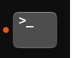
\includegraphics[width=0.1\linewidth]{VM/5.png}
\caption{Терминал.}
\label{ris:image}
\end{figure}

\begin{figure}
\quad Для скачивания чего-либо необходимо ввести соответствующие строки коды:
\newline git – sudo apt install git
\newline nodejs – sudo apt install nodejs
\newline npm - sudo apt install npm
\newline grunt - sudo apt install grunt
\newline Чтобы удостовериться, что всё правильно скачалось, можно узнать версию данного продукта. Например: git –version
\end{figure}

\begin{figure}
\quad 2.\quad  Регистрация на github.
\newline \quad Для регистрации на github нужно перейти по ссылке: : https://github.com/ и заполнить всю необходимую информацию о себе.
\end{figure}

\begin{figure}
\quad     3. \quad Работа с репозиторием.
\newline \quad Переходим по ссылке: https://github.com/nickkolok/chas-ege/. Далее нажимаем на зелёную кнопку с надписью «Code», и копируем ссылку репозитория. Лучше сделать это сразу, потому что «Ubuntu» на «VirtualBox» может сильно нагружать компьютер, и открыть вкладку с браузером может быть проблематично из-за нагрузки. (Если возникли проблемы с копирование ссылки, то попробуйте открыть браузер внутри «Ubuntu», перейти по ссылке и скопировать ссылку репозитория в нём.)

		\centering
		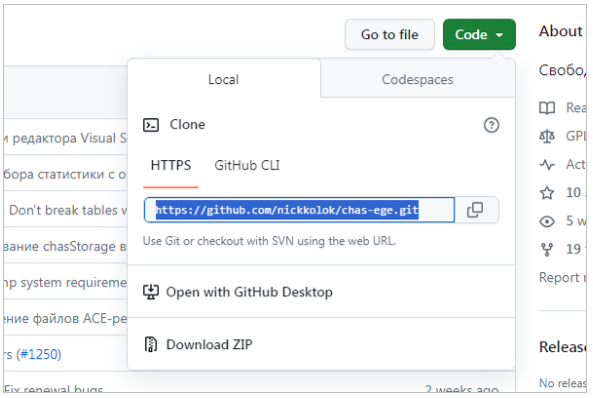
\includegraphics[width=0.65\linewidth]{VM/6.png}
\caption{Github. Ссылка на репозиторий.}
\label{ris:image}
\end{figure}

\begin{figure}
• Далее снова заходим в терминал и создаём папку на рабочем столе командой: mkdir <название папки>. Можете убедиться, что папка создана, с помощью команды: ls. Вы увидите все папки на рабочем столе, среди которых должна быть ваша, только что созданная.Затем зайдите в папку командой: cd <название папки>, и клонируйте себе репозиторий командой: git clone <ссылка на репозиторий >
  \newline   • Добавляем себе ссылку на основной репозиторий проекта с помощью команды: git remote add upstream <ссылка на репозиторий > и убеждаемся, что он подключился, командой: git fetch upstream
   \newline  • Собираем проект командой: grunt. Важно выполнять эту команду в папке, в которую мы и склонировали репозиторий.
  \newline  • Открываем файл dist/sh/otladka.html в браузере командой: open otladka.html


		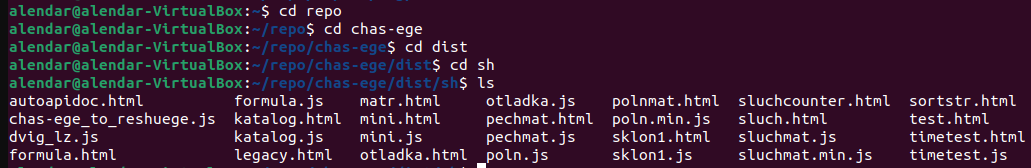
\includegraphics[width=1\linewidth]{VM/7.png}
\caption{Путь к файлу otladka.html.}
\label{ris:image}
\quad Запускаем любой шаблон, для проверки, в открывшемся окне.
\end{figure}
